%!TEX root = /Users/stevenmartell/Documents/CURRENT PROJECTS/iSCAM-trunk/fba/BC-herring-2011/WRITEUP/BCHerring2011.tex
\section{Technical description of \iscam}\label{appiSCAM}
%%%%%%%%%%%%%%%%%%%%%%%%%%%%%%%%%%%%%%%%%%%%%%%%%%%%%%%%%%%%%%%%%%%%%
%%%%%%%%%%%%%%%%%%%%%%%%%%%%%%%%%%%%%%%%%%%%%%%%%%%%%%%%%%%%%%%%%%%%%	
%%      Move to appendix  
	\subsection{Analytic methods}
	The section contains the documentation in mathematical form of the underlying age structured model, and its steady state version that is used to calculate MSY-based reference points, the observation models used in predicting observations, and the components of the objective function that formulate the statistical criterion that is used to estimate model parameters. All of the model equations are laid out in tables and are intended to represent the order of operations, or pseudocode, in which to implement the model. \iscam was implemented in AD Model Builder version 10.1 \citep{ADMB2009}.  This appendix also describes some of the optional features in \iscam\ for estimating nonparametric selectivities.  
	
	It should be noted here that MSY-based reference points assume steady-state conditions, and the model structure that is implemented for the BC herring stocks is non-stationary due to time-varying changes in natural mortality rates ($M_t$) and selectivity.  Estimates of MSY are conditional on the estimates of $M$, selectivity and mean weight-at-age; all of which change over time in the herring assessments.  In the calculations of reference points, we use the average natural mortality between 1951-2010 and estimated selectivities and the empirical weight-at-age data in 2011.

\subsection{Equilibrium considerations}

Steady-state conditions are presented in Table \ref{Table2}, in here we assume the parameter vector $\Theta$ in \eqref{T2.1} is unknown (with the exception of $F_e$) and would eventually be estimated by fitting \iscam\ to time series data. The definition of $F_e$ is the steady-state fishing mortality rate, and the value of $F_e$ that maximizes equilibrium yield corresponds to \fmsy\ (see section \ref{sec:Finding_MSY}).   For a given set of growth parameters (or if available empirical weight-at-age data) and maturity-at-age parameters defined by \eqref{T2.3}, growth is assumed to follow the von Bertalanffy model \eqref{T2.4}, mean weight-at-age is given by the allometric relationship in \eqref{T2.5}, and the age-specific vulnerability is given by a logistic function \eqref{T2.6}.  Note, however, there are alternative selectivity functions implemented in \iscam, the logistic function used here is simply for demonstration purposes.  Mean fecundity-at-age is assumed to be proportional to the mean weight-at-age of mature fish, where maturity at age is specified by the parameters $\dot{a}$ and $\dot{\gamma}$ for the logistic function.

 

%%%%%%%%%%%%%%%%%%%%%%%%%%%%%%%%%%%%%%%%%%%%%%%%%%%%%%%%%%%%%%%%%%%%%%
%%%%%%%%%%%%%%%%%%%%%%%%%%%%%%%%%%%%%%%%%%%%%%%%%%%%%%%%%%%%%%%%%%%%%%
\begin{table}[!tbp]
  %\centering
\caption{Steady-state age-structured model assuming unequal
vulnerability-at-age, age-specific natural mortality, age-specific
fecundity and Beverton-Holt type recruitment.  Note that $M$ is the average natural mortality rate between 1951-2011.}\label{Table2} 
\tableEq
    \begin{gather}
           \hline
        \mbox{Parameters} \nonumber \\
            \Theta = (B_o,\kappa,M,\hat{a},\hat{\gamma},F_e) \label{T2.1}\\
            B_o>0; \kappa > 1; M > 0; F_e \ge 0 \nonumber\\
            \Phi = (l_\infty, k, t_o,a,b,\dot{a},\dot{\gamma}) \label{T2.3}\\[1ex]
        %%
        %%
        \mbox{Age-schedule information} \nonumber\\
            l_a=l_\infty(1-\exp(-k(a-t_o)))\label{T2.4}\\
            w_a=a(l_a)^b \label{T2.5}\\
            v_a=(1+\exp(-(\hat{a}-a)/\gamma))^{-1} \label{T2.6}\\
            f_a=w_a(1+\exp(-(\dot{a}-a)/\dot{\gamma}))^{-1} \label{T2.7}\\[1ex]
        %%
        %%
        \mbox{Survivorship} \nonumber\\
            \iota_a=\begin{cases} 1, \quad a=1      \label{T2.8} \\
            \iota_{a-1}e^{-M},\quad a>1\\
            \iota_{a-1}/(1-e^{-M}),\quad a=A \end{cases}\\
            \hat{\iota}_a=\begin{cases} 1, \quad a=1\\
            \hat{\iota}_{a-1}e^{-M-F_e v_{a-1}},\quad a>1\\
            \hat{\iota}_{a-1}e^{-M-F_e v_{a-1}}/(1-e^{-M-F_e v_{a}}),\quad a=A
            \end{cases} \label{T2.9}\\[1ex]
        %%
        %%
        \mbox{Incidence functions} \nonumber \\
            \phi_E=\sum_{a=1}^\infty \iota_a f_a, \quad
            \phi_e=\sum_{a=1}^\infty \hat{\iota}_a f_a \label{T2.10}\\
            \phi_B=\sum_{a=1}^\infty \iota_a w_a v_a, \quad
            \phi_b=\sum_{a=1}^\infty \hat{\iota}_a w_a v_a \label{T2.11}\\
            \phi_q=\sum_{a=1}^\infty
                \frac{ \hat{\iota}_a w_a v_a}{M+F_ev_a}
                \left(1-e^{(-M-F_ev_a)}\right) \label{T2.11b} \\[1ex]
        %%
        %%
        \mbox{Steady-state conditions} \nonumber \\
        R_o=B_o/ \phi_B \label{T2.12}\\
        R_e=R_o\frac{\kappa-\phi_E/\phi_e}{\kappa-1} \label{T2.13}\\
        %%C_e=R_e \phi_b \frac{F_e}{Z_e}(1-\exp(-Z_e))\label{T2.14} \B \\
        C_e=F_e R_e \phi_q\label{T2.14} \\[1ex]
        \hline \hline \nonumber
    \end{gather}
    \normalEq
\end{table}
%%%%%%%%%%%%%%%%%%%%%%%%%%%%%%%%%%%%%%%%%%%%%%%%%%%%%%%%%%%%%%%%%%%%%%
%%%%%%%%%%%%%%%%%%%%%%%%%%%%%%%%%%%%%%%%%%%%%%%%%%%%%%%%%%%%%%%%%%%%%%
Survivorship for unfished and fished populations is defined by \eqref{T2.8} and \eqref{T2.9}, respectively.  It is assumed that all individuals ages $A$ and older (i.e., the plus group) have the same total mortality rate.  The incidence functions refer to the life-time or per-recruit quantities such as spawning biomass per recruit ($\phi_E$) or vulnerable biomass per recruit ($\phi_b$).  Note that upper and lower case subscripts denote unfished and fished conditions, respectively.  Spawning biomass per recruit is given by \eqref{T2.10}, the vulnerable biomass per recruit is given by \eqref{T2.11} and the per recruit yield to the fishery is given by \eqref{T2.11b}.  Unfished recruitment is given by \eqref{T2.12} and the steady-state equilibrium recruitment  for a given fishing mortality rate $F_e$ is given by \eqref{T2.13}.  Note that in \eqref{T2.13} we assume that recruitment follows a Beverton-Holt model of the form:
\[
R_e=\frac{s_o R_e \phi_e}{1+\beta R_e \phi_e}
\]
where
\[
s_o = \kappa/\phi_E,
\]
\[
\beta = \frac{(\kappa-1)}{R_o\phi_E},
\]
which simplifies to \eqref{T2.13}.
The equilibrium yield for a given fishing mortality rate is \eqref{T2.14}.  These steady-state conditions are critical for determining various reference points such as \fmsy\ and \bmsy. The description of calculating steady-state yield for a given value of $F_e$ in Table \ref{Table2} is written assuming that only one fishing fleet exists.  The actual calculations are slightly more complicated for the BC herring fishery, as there are three distinct fishing fleets that each have different selectivities.  The actual selectivities and calculations of survivorship involve a matrix of age-specific fishing mortalities, where each row of this matrix corresponds to one fishing fleet.  In this case $F_e$ is the total fishing mortality rate for fully selected fish summed over all fleets.  In order to calculate the fleet specific fishing mortality rate, a fixed allocation of the total yield must be specified \textit{a priori}.
	
\subsection{MSY based reference points}\label{sec:Finding_MSY}
\iscam\ calculates MSY-based reference points by finding the value of $F_e$ that results in the zero derivative of the steady-state catch equation \eqref{T2.14}.  This is accomplished numerically using a Newton-Raphson method where an initial guess for \fmsy\ is set equal to 1.5$M$, then use \eqref{eq1.1} to iteratively find \fmsy.  Note that the partial derivatives in \eqref{eq1.1} can be found in Table \ref{Table3}.

\begin{align}\label{eq1.1}
    F_{e+1}&=F_e - 
    \dfrac{ \dfrac{\partial C_e}{\partial F_e}}
    { \dfrac{\partial^2 C_e}{\partial F_e}}\\
    \mbox{where}\nonumber\\
     \frac{\partial C_e}{\partial F_e} &=
    R_e \phi_q
    + F_e \phi_q \dfrac{\partial R_e}{\partial F_e}
    + F_e R_e \dfrac{\partial \phi_q}{\partial F_e} \nonumber\\
    \frac{\partial^2 C_e}{\partial F_e} &=
    \phi_q \dfrac{\partial R_e}{\partial F_e}
   +  R_e \dfrac{\partial \phi_q}{\partial F_e}\nonumber
%    \frac{R_e \phi_q
%    + F_e \phi_q \dfrac{\partial R_e}{\partial F_e}
%    + F_e R_e \dfrac{\partial \phi_q}{\partial F_e}}
%    {\phi_q \dfrac{\partial R_e}{\partial F_e}
%    +  R_e \dfrac{\partial \phi_q}{\partial F_e}}.
\end{align}

The algorithm usually converges in less than 10 iterations depending on how close the initial guess of \fmsy\ is to the true value.  A maximum of 20 iterations are allowed in \iscam, however, if $\frac{\partial C_e}{\partial F_e}<10^{-5}$ the algorithm stops.  Note also, that this is only performed on data type variables and not differentiable variables within AD Model Builder.

Given an estimate of \fmsy, other reference points such as MSY are calculated use the equations in Table \ref{Table2} where each of the expressions is evaluated at \fmsy.  A graphical representation of MSY based reference points for two alternative values of the recruitment compensation parameter $\kappa$ is show in Figure \ref{FigMSY}.

\begin{figure}[!tbp]
  % Requires \usepackage{graphicx}
  \centering
  \includegraphics[width=0.5\columnwidth]{../Figs/Fig1Quadplot.pdf}\\
  \caption{Equilibrium yield (a), recruits (b), biomass (c) and
spawner per recruit ($\phi_e/\phi_E$) (d) versus instantaneous
fishing mortality $F_e$ for two different values of the recruitment
compensation ratio ($\kappa=12$ solid lines, $\kappa=4$ dashed
lines). Vertical lines in each panel correspond to \fmsy\ and
horizontal lines correspond to various reference points that would
achieve MSY.}\label{FigMSY}
\end{figure}

%% Add bit here about how reference points are calculated when there
%% are multiple gears with different selectivities.  Also how this is
%% done when using empirical body weight data.

There are some additional technical details about calculating MSY based reference points when considering multiple fishing gears with different selectivities.  The maximum sustainable yield summed over all fishing gears is a function of the selectivities of each gear type and what fraction of the total catch is allocated to each gear.  In the Pacific herring fishery, there are three distinct fleets that all have different selectivities; the purse-seine gears tend to catch smaller younger fish, while the gill net fishery tends to target larger mature females.  The optimum fishing mortality rate for each gear that would maximize the yield depends on what the other gears are removing; this in itself is another optimization problem that fisheries management must contend with.  For the purposes of this assessment, \iscam\ requires an allocation of the total catch (summed across gear type) to each gear before it proceeds with calculating reference points.

For this herring assessment, the average catch over the past 20 years used to determine the allocation scheme for each of the stock assessment regions.  For the Strait of Georgia this corresponds to 6.9\% for the winter seine fishery, 41.4\% for the seine roe fishery, and 51.8\% for the gill net fishery.  We further assume that 100\% of the total mortality takes place prior to spawning, and the start of each biological year is the month of April.


%%%%%%%%%%%%%%%%%%%%%%%%%%%%%%%%%%%%%%%%%%%%%%%%%%%%%%%%%%%%%%%%%%%%%%
%%%%%%%%%%%%%%%%%%%%%%%%%%%%%%%%%%%%%%%%%%%%%%%%%%%%%%%%%%%%%%%%%%%%%%
\begin{table}
  \centering
\caption{Partial derivatives, based on components in Table
\ref{Table2}, required for the numerical calculation of \fmsy\ using \eqref{eq1.1}.}\label{Table3} \tableEq
    \begin{gather}
        \hline
        \mbox{Mortality \& Survival} \nonumber \\
        Z_{a}=M+F_ev_a \label{T3.1} \\
        S_{a}=1-e^{-Z_a}\label{T3.2}\\[1ex]
        %%
        %%
        \mbox{Partial for survivorship} \nonumber \\
        \frac{\partial \hat{\iota}_a}{\partial F_e} =
        \begin{cases}
          0,& a=1 \label{T3.3}\\
          e^{-Z_{a-1}}\left(\dfrac{\partial \hat{\iota}_{a-1}}{\partial F_e}
           -\hat{\iota}_{a-1}v_{a-1}\right),& 1<a<A\\
           \dfrac{\dfrac{\partial \hat{\iota}_{a-1}}{\partial F_e}}
           {(1-e^{-Z_a})} -
           \dfrac{\hat{\iota}_{a-1} e^{-Z_{a-1}} v_a e^{-Z_a}}
           {(1-e^{-Z_a})^2}, &a=A
        \end{cases} \\[1ex]
        %%
        %%
        \mbox{Partials for incidence functions} \nonumber \\
        \frac{\partial \phi_e}{\partial F_e}=
            \sum_{a=1}^\infty f_a \frac{\partial \hat{\iota}_a}{\partial F_e} \label{T3.4}\\
        %%
        %%
        \frac{\partial \phi_q}{\partial F_e}=
            \sum_{a=1}^\infty \frac{w_av_a S_a}{Z_a}
             \frac{\partial \hat{\iota}_a}{\partial F_e}
             +\frac{\hat{\iota}_a w_av_a^2}{Z_a}\left(e^{-Z_a}-\frac{S_a}{Z_a} \right) \label{T3.5}\\[1ex]
        %%
        %%
        \mbox{Partial for recruitment} \nonumber\\
        \frac{\partial R_e}{\partial F_e}=\frac{R_o}{\kappa-1}
        \frac{\phi_E}{\phi_e^2} \frac{\partial \phi_e}{\partial
        F_e} \label{T3.6}\\[1ex]
        \hline \hline \nonumber
    \end{gather}

    \normalEq
\end{table}
%%%%%%%%%%%%%%%%%%%%%%%%%%%%%%%%%%%%%%%%%%%%%%%%%%%%%%%%%%%%%%%%%%%%%%
%%%%%%%%%%%%%%%%%%%%%%%%%%%%%%%%%%%%%%%%%%%%%%%%%%%%%%%%%%%%%%%%%%%%%%
	
		
		\subsection{Dynamic age-structured model}

The estimated parameter vector in \iscam\ is defined in \eqref{T4.1}, where $R_0, \kappa$ and $M$ are the leading unknown population parameters that define the overall population scale in the form of unfished recruitment and productivity in the form of recruitment compensation and natural mortality.  The total variance $\vartheta^2$ and the proportion of the total variance that is associated with observation errors $\rho$ are also estimated, then the variance is partitioned into observation errors ($\sigma^2$) and process errors ($\tau^2$) using \eqref{T4.2}.

The unobserved state variables \eqref{T4.3} include the numbers-at-age year year $t$ ($N_{t,a}$), the spawning stock biomass ($B_t$) and the total age-specific total mortality rate ($Z_{t,a}$).

The initial numbers-at-age in the first year \eqref{T4.4} and the annual recruits \eqref{T4.5} are treated as estimated parameters and used to initialize the numbers-at-age matrix.  Age-specific selectivity for gear type $k$ is a function of the selectivity parameters $\gamma_k$ \eqref{T4.6}, and the annual fishing mortality for each gear $k$ in year $t$ ($\digamma_{k,t}$).  The vector of log fishing mortality rate parameters $\digamma_{k,t}$ is a bounded vector with a minimum value of -30 and an upper bound of 3.0.  In arithmetic space this corresponds to a minimum value of 9.36e-14 and a maximum value of 20.01 for annual fishing mortality rates.  In years where there are 0 reported catches for a given fleet, no corresponding fishing mortality rate parameter is estimated and the implicit assumption is there was no fishery in that year.

There is an option to treat natural mortality as a random walk process \eqref{T4.6b}, where the natural mortality rate in the first year is the estimated leading parameter \eqref{T4.1} and in subsequent years the mortality rate deviates from the previous year based on the estimated deviation parameter $\varphi_t$.  If the mortality deviation parameters are not estimated, then $M$ is assumed to be time invariant. 



%%%%%%%%%%%%%%%%%%%%%%%%%%%%%%%%%%%%%%%%%%%%%%%%%%%%%%%%%%%%%%%%%%%%%%%%
%%%%%%%%%%%%%%%%%%%%%%%%%%%%%%%%%%%%%%%%%%%%%%%%%%%%%%%%%%%%%%%%%%%%%%%%
\begin{table}[!tpb]
  \centering
\caption{Statistical catch-age model using the Baranov catch
equation, where $R_0$ and $\kappa$ are the leading parameters that define population scale and productivity, respectively.}\label{Table4}
\tableEq
    \begin{align}
        \hline \nonumber \\
        &\mbox{Estimated parameters} \nonumber\\
        \begin{split}
        \Theta&= 
        		\left(R_0,\kappa,M,\bar{R},\ddot{R},\rho,\vartheta,
		\vec{\gamma}_{k}
				,\digamma_{k,t}, %\delta_{k,t},
		 \{\ddot{\omega}_a\}_{a=\acute{a}+1}^{a=A},
		 \{\omega_t\}_{t=1}^{t=T},
        		\{\varphi_t \}_{t=2}^T\right)
	\end{split} \label{T4.1}\\
        \sigma&=\rho /\vartheta, \quad
        \tau=(1-\rho)/\vartheta\label{T4.2}\\[1ex]
        %\vartheta^2=\sigma^2+\tau^2, \quad
        %\rho=\frac{\sigma^2}{\sigma^2+\tau^2}\label{T4.3}\\[1ex]
        %%
        %%
        &\mbox{Unobserved states} \nonumber\\
        &N_{t,a},B_t,Z_{t,a}	\label{T4.3}\\
	%%
	%%	        
        &\mbox{Initial states ($t=\acute{t}$)} \nonumber\\
        %v_a=\left[1+e^{-(\hat{a}-a)/\hat{\gamma}}\right]^{-1}\label{T4.7}\\
        N_{t,a}&=\ddot{R}e^{\ddot{\omega}_{a}} \exp(-M_t)^{(a-\acute{a})};
        	\quad t=\acute{t};  \acute{a}\leq a\leq A \label{T4.4}\\
        N_{t,a}&=\bar{R}e^{\omega_{t}} ;\quad \acute{t}\leq t\leq T;  
        	a=\acute{a} \label{T4.5}\\
        v_{k,a}&=f(\vec{\gamma}_k) \label{T4.6}\\
        M_t &= M_{t-1} \exp(\varphi_t), \quad t>1, \varphi_t \sim N(0,\sigma_M) \label{T4.6b}\\
        F_{k,t}&= \exp(\digamma_{k,t}) \label{T4.7}\\[1ex]
        %%F_{k,t}&=\bar{F}_k \exp(\delta_{k,t}) \label{T4.7}\\[1ex]
        %%
        %%
        &\mbox{State dynamics ($t>\acute{t}$)} \nonumber\\
        B_t&=\sum_a N_{t,a}f_a \label{T4.8}\\
        Z_{t,a}&=M_t+\sum_k F_{k,t} v_{k,t,a}\label{T4.9}\\
        \hat{C}_{k,t}&=\sum _ a\frac {N_{{t,a}}w_{{a}}F_{k,t} v_{{k,t,a}}
        \left( 1-{e^{-Z_{t,a}}} \right) }{Z_{t,a}} e^{\eta_t} \label{T4.10}\\
        %F_{t_{i+1}}= \ F_{t_{i}} -\frac{\hat{C}_t-C_t}{\hat{C}_t'} \label{T4.12}\\
        N_{t,a}&=\begin{cases}
            %\dfrac{s_oE_{t-1}}{1+\beta E_{t-1}} \exp(\omega_t-0.5\tau^2) &a=1\\ \\
            N_{t-1,a-1} \exp(-Z_{t-1,a-1}) &a>\acute{a}\\
            N_{t-1,a} \exp(-Z_{t-1,a}) & a=A
        \end{cases}\label{T4.11}\\[1ex]
        %%
        %%
        &\mbox{Recruitment models} \nonumber\\
        R_t &= \frac{s_oB_{t-k}}{1+\beta B_{t-k}}e^{\delta_{t}-0.5\tau^2}\label{T4.12}
        	\quad \mbox{Beverton-Holt}  \\
        R_t &= s_oB_{t-k}e^{-\beta B_{t-k}+\delta_t-0.5\tau^2}\label{T4.13}
        	\quad \mbox{Ricker} \\
	%%        \mbox{Residuals \& predicted observations} \nonumber\\
	%%        \epsilon_t=\ln\left(\frac{I_t}{B_t}\right)-\frac{1}{n}\sum_{t \in I_t}\ln\left(\frac{I_t}{B_t}\right)\label{T4.15}\\
	%%        \hat{A}_{t,a}=\dfrac{N_{t,a}\dfrac{F_tv_a}{Z_{t,a}}\left(1-e^{-Z_{t,a}}\right)}
	%%        {\sum_a N_{t,a}\dfrac{F_tv_a}{Z_{t,a}}\left(1-e^{-Z_{t,a}}\right)}\label{T4.16}\\
        \hline \hline \nonumber
    \end{align}

    \normalEq
\end{table}
%%%%%%%%%%%%%%%%%%%%%%%%%%%%%%%%%%%%%%%%%%%%%%%%%%%%%%%%%%%%%%%%%%%%%%%%
%%%%%%%%%%%%%%%%%%%%%%%%%%%%%%%%%%%%%%%%%%%%%%%%%%%%%%%%%%%%%%%%%%%%%%%%

%% Make into a longtable.
\begin{table}[htdp]
\caption{An incomplete list of symbols, constants and description for variables used in \iscam.}\label{TableSymbols}
\begin{center}
\begin{tabular}{lcl}
\hline
Symbol & Constant value & Description\\
\hline
\multicolumn{3}{l}{\underline{Indexes}}\\
a & & index for age\\
t & & index for year\\
k & & index for gear\\
\multicolumn{3}{l}{\underline{Model dimensions}}\\
$\acute{a}, A$ & 2, 10& youngest and oldest age class ($A$ is a plus group)\\
$\acute{t}, T$ & 1951, 2010 & first and last year of catch data\\
$K$ & 5 & Number of gears including survey gears\\
\multicolumn{3}{l}{\underline{Observations (data)}}\\
$C_{k,t}$ & & catch in weight by gear $k$ in year $t$\\
$I_{k,t}$ & & relative abundance index for gear $k$ in year $t$\\
$p_{k,t,a}$& & observed proportion-at-age $a$ in year $t$ for gear $k$\\
\multicolumn{3}{l}{\underline{Estimated parameters}}\\
$R_o$ & & Age-$\acute{a}$ recruits in unfished conditions\\
$\kappa$ & & recruitment compensation\\
$M$ & & instantaneous natural mortality rate \\
$\bar{R}$ & & average age-$\acute{a}$ recruitment from year $\acute{t}$ to $T$\\
$\ddot{R}$ & & average age-$\acute{a}$ recruitment in year $\acute{t}-1$\\
$\rho$ & & fraction of the total variance associated with observation error\\
$\vartheta$ & & total precision (inverse of variance) of the total error\\
$\vec{\gamma}_k$ & & vector of selectivity parameters for gear $k$\\
$\digamma_{k,t}$ & & logarithm of the instantaneous fishing mortality for gear $k$ in year $t$\\
$\ddot{\omega}_a$&& age-$\acute{a}$ deviates from $\ddot{R}$ for year $\acute{t}$\\
$\omega_t$&& age-$\acute{a}$ deviates from $\bar{R}$ for years $\acute{t}$ to $T$\\
$\varphi_t$&& logarithm of annual change in natural mortality rate\\
\multicolumn{3}{l}{\underline{Standard deviations}}\\
$\sigma_M$ &0.1& standard deviation in random walk for natural mortality\\
$\sigma$ && standard deviation for observation errors in survey index\\
$\tau$ && standard deviation in process errors (recruitment deviations)\\
$\sigma_C$& 0.0707 & standard deviation in observed catch by gear\\
\multicolumn{3}{l}{\underline{Residuals}}\\
$\delta_t$ && annual recruitment residual\\
$\eta_t$ && residual error in predicted catch\\
\hline \hline
\end{tabular}
\end{center}
\end{table}%


State variables in each year are updated using equations \ref{T4.8}--\ref{T4.11}, where the spawning biomass is the product of the numbers-at-age and the mature biomass-at-age \eqref{T4.8}.  The total mortality rate is given by \eqref{T4.9}, and the total catch (in weight) for each gear is given by \eqref{T4.10} assuming that both natural and fishing mortality occur simultaneously throughout the year.  The numbers-at-age are propagated over time using \eqref{T4.11}, where members of the plus group (age $A$) are all assumed to have the same total mortality rate.  

Recruitment to age $k$ can follow either a Beverton-Holt model \eqref{T4.12} or a Ricker model \eqref{T4.13} where the maximum juvenile survival rate ($s_o$) in either case is defined by $s_o=\kappa/\phi_E$.  For the Beverton-Holt model, $\beta$ is derived by solving \eqref{T4.12} for $\beta$ conditional on estimates of $\kappa$ and $R_o$:
\[
\beta = \frac{\kappa-1}{R_o \phi_E},
\]
and for the Ricker model this is given by:
\[
\beta = \frac{\ln(\kappa)}{R_o \phi_E}
\]


		
\subsection{Options for selectivity}\label{Appendix:SelectivityOptions}
		
At present, there are eight alternative age-specific selectivity options in \iscam.  The simplest of the selectivity options is a simple logistic function with two parameters where it is assumed that selectivity is time-invariant.  The more complex selectivity options assume that selectivity may vary over time a may have as many as (A-1)$\cdot$T parameters.  For time-varying selectivity, cubic and bicubic splines are used to reduce the number of estimated parameters. The last two options consider how selectivity may vary over time based on changes in mean weight-at-age. Prior to parameter estimation, \iscam\ will determine the exact number of selectivity parameters that need to be estimated based on which selectivity option was chosen for each gear type.  It is not necessary for all gear types to have the same selectivity option.  For example it is possible to have a simple two parameter selectivity curve for say a survey gear, and a much more complicated selectivity option for a commercial fishery.

\paragraph{Logistic selectivity} 
The logistic selectivity option is a two parameter model of the form
\[
v_a = \frac{1}{1+ \exp{(-(a-\mu_{a})/\sigma_a)}}
\]
where $\mu_a$ and $\sigma_a$ are the two estimated parameters representing the age-at-50\% vulnerability and the standard deviation, respectively.

\paragraph{Age-specific selectivity coefficients}
The second option also assumes that selectivity is time-invariant and estimates at total of $A$-1 selectivity coefficients, where the plus group age-class is assumed to have the same selectivity as the previous age-class.  For example, if the ages in the model range from 1 to 15 years, then a total of 14 selectivity parameters are estimated, and age-15+ animals will have the same selectivity as age-14 animals.

When estimating age-specific selectivity coefficients, there are two additional penalties that are added to the objective function that control how much curvature there is and limit how much dome-shaped can occur.  To penalize the curvature, the square of the second differences of the vulnerabilities-at-age are added to the objective function: 
\begin{equation}\label{eq2ndDiff}
\lambda_k^{(1)} \sum_{a=2}^{A-1}(v_{k,a} - 2v_{k,a-1} + v_{k,a-2})^2
\end{equation}
The dome-shaped term penalty as:
\begin{equation}\label{eqDomePenalty}
\begin{cases}
\lambda_k^{(2)} \sum_{a=1}^{A-1}(v_{k,a} - v_{k,a+1})^2& \mbox(if) v_{k,a+1}< v_{k,a}\\
0 & \mbox(if) v_{k,a+1}\geq v_{k,a}
\end{cases}
\end{equation}
For this selectivity option the user must specify the relative weights ($\lambda_k^{(1)},\lambda_k^{(2)}$) to add to these two penalties.

\paragraph{Cubic spline interpolation}
The third option also assumes time-invariant selectivity and estimates a selectivity coefficients for a series age-nodes (or spline points) and uses a natural cubic spline to interpolate between these nodes (Figure \ref{Fig2}). Given $n+1$ distinct knots $x_i$, selectivity can be interpolated in the intervals defined by
\[
S(x) = \begin{cases}
	S_0(x) & x \in [x_0,x_1]\\
	S_1(x) & x \in [x_1,x_2]\\
	...\\
	S_{n-1}(x) & x \in [x_{n-1},x_n]
\end{cases}
\]
where  $S''(x_0) = S''(x_n)=0$  is the condition that defines a natural cubic spline.
\begin{figure}
	\centering
	% Requires \usepackage{graphicx}
	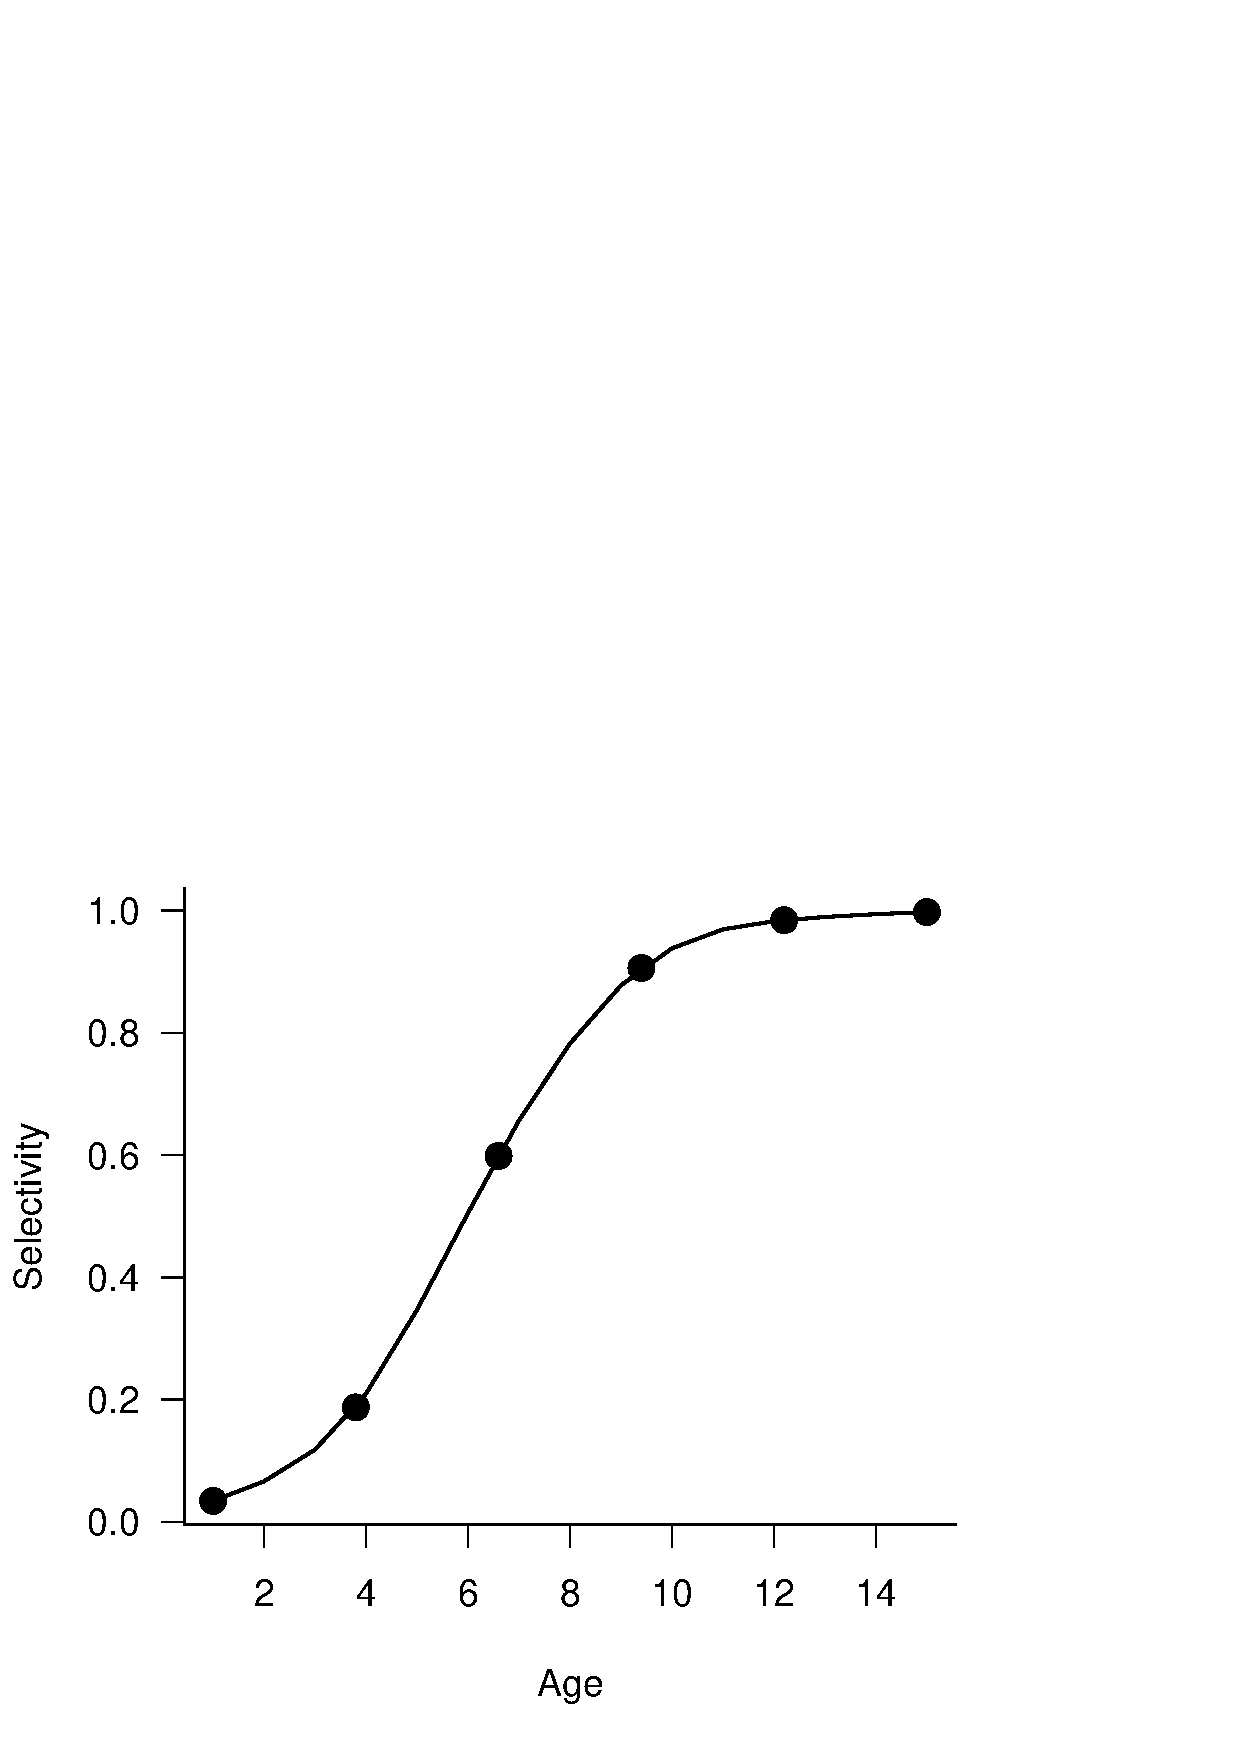
\includegraphics[width=0.4\columnwidth]{../Figs/SplineEg.pdf}\\
	\caption{Example of a natural cubic spline interpolation for 15-selectivity coefficients based on estimating 6 nodes (true selectivity was based on a logistic function).  In \iscam\ the user specifies the number of nodes (e.g., 6 circles) to estimate; then the 15 age-specific selectivity coefficients are interpolated using a natural cubic spline.}\label{Fig2}
\end{figure}

The same penalty functions for curvature and dome-shaped selectivity are also invoked for the cubic spline interpolation of selectivity.

\paragraph{Time-varying selectivity with cubic spline interpolation} A fourth option allows for cubic spline interpolation for age-specific selectivity  in each year.  This option adds a considerable number of estimated parameters but the most extreme flexibility.  For example, given 40 years of data and estimated 5 age nodes, this amounts 200 (40 years times 5 ages) estimated selectivity parameters.  Note that the only constraints at this time are the dome-shaped penalty and the curvature penalty; there is no constraint implemented for say a random walk (first difference) in age-specific selectivity).  As such this option should only be used in cases where age-composition data is available for every year of the assessment.

\paragraph{Bicubic spline to interpolate over time and ages}  The fifth option allows for a two-dimensional interpolation using a bicubic spline (Figure \ref{Fig3}).  In this case the user must specify the number of age and year nodes.  Again the same curvature and dome shaped constraints are implemented.  It is not necessary to have age-composition data each and every year as in the previous case, as the bicubic spline will interpolate between years.  However, it is not advisable to extrapolate selectivity back in time or forward in time where there are no age-composition data unless some additional constraint, such as a random-walk in age-specific selectivity coefficients is implemented (as of \today, this has not been implemented).

\begin{figure}[!tbp]
	% Requires \usepackage{graphicx}
	\centering
	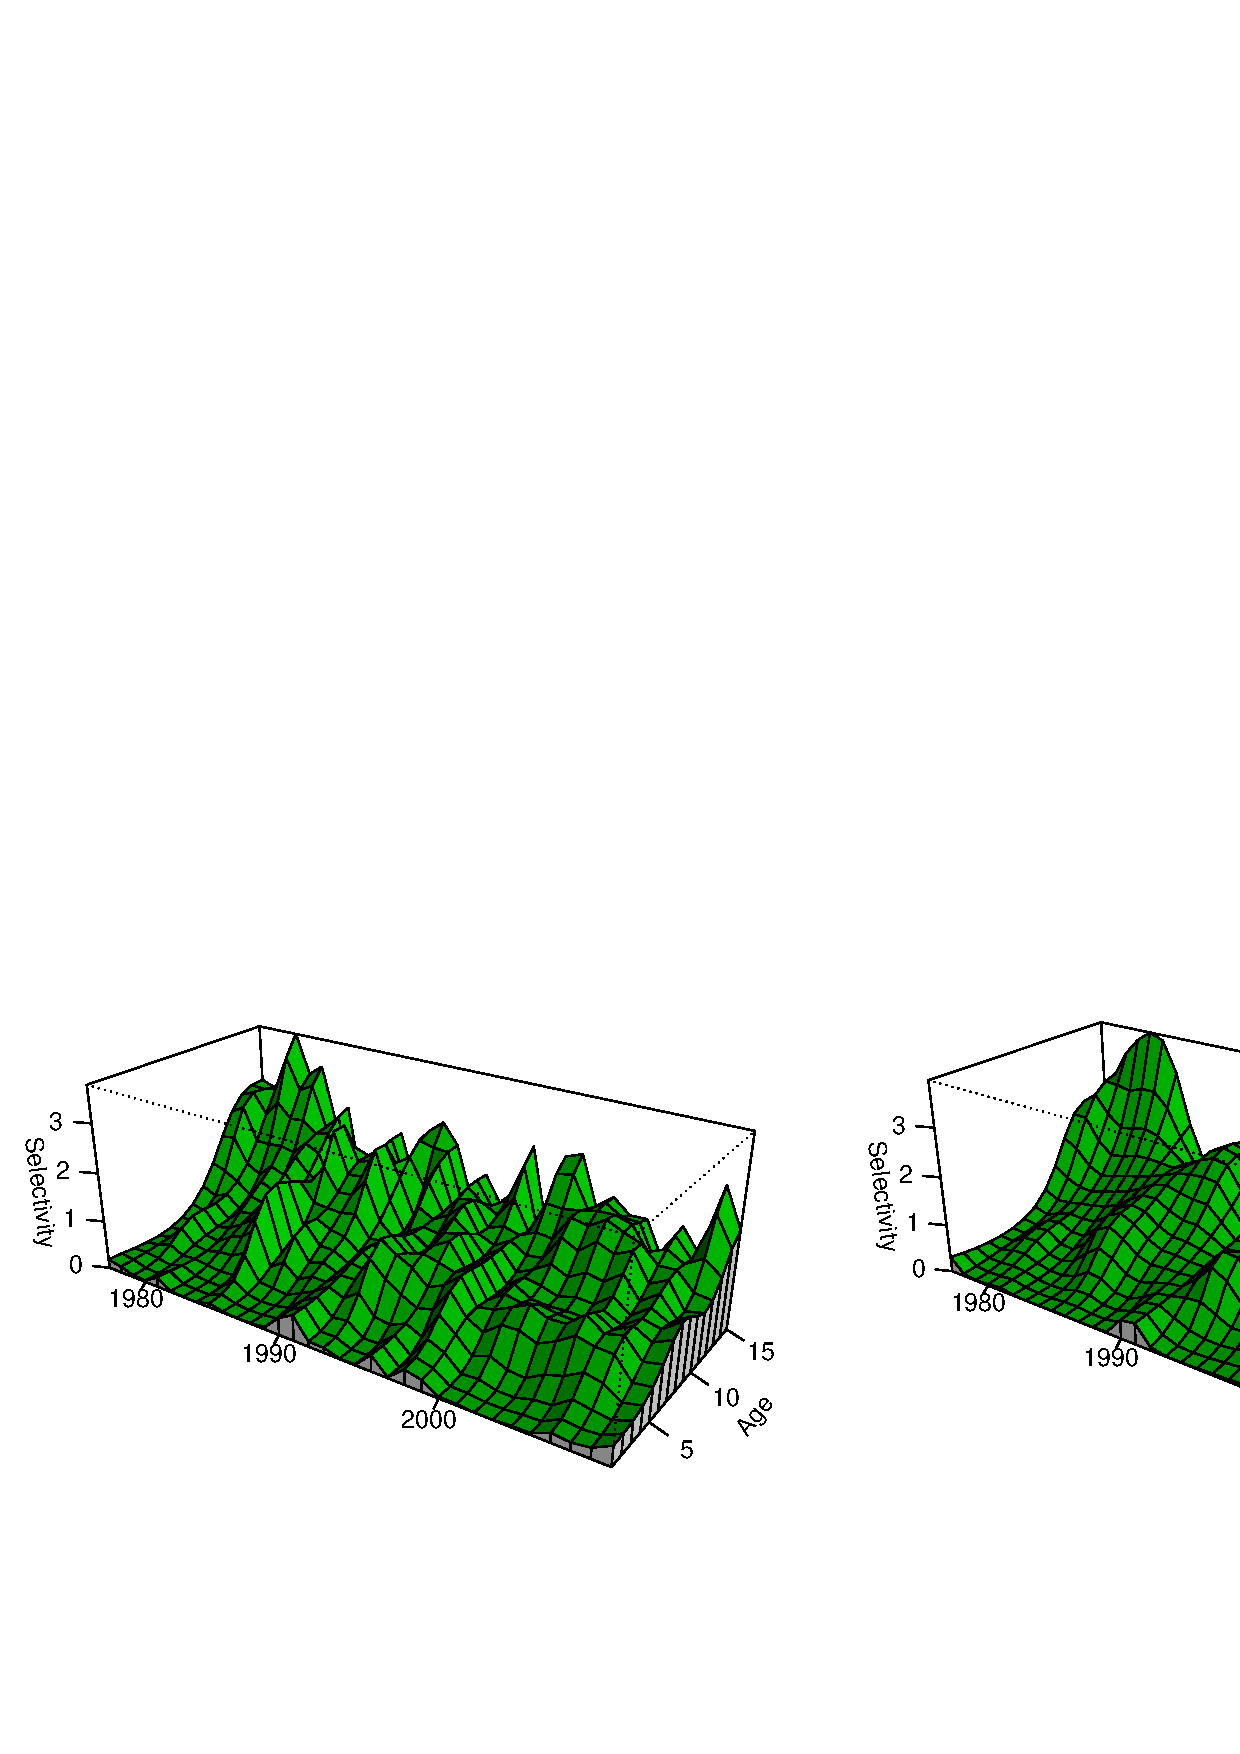
\includegraphics[width=0.9\textwidth]{../Figs/BicubicEg.pdf}\\
	\caption{Example of a time-varying cubic spline (left) and bicubic spline (right) interpolation for selectivity based on data from the Pacific hake. The panel on the left contains 165 estimated selectivity parameters and the bicubic interpolation estimates 85 selectivity parameters, or 5 age nodes and 17 year nodes. There are 495 actual nodes (selectivity parameters) being interpolated.}\label{Fig3}
\end{figure}


\paragraph{Selectivity as a logistic function of weight-at-age}

The seventh option for selectivity is to parameterize a logistic function in terms of the weight-at-age in year $t$ ($w_{a,t}$). In this case changes in weight-at-age over time allow for changes in selectivity. Such a weight-based function may be appropriate for size selective gears such as gill nets. 
\[
v_{a,t} = \frac{1}{1+ \exp{(-(w_{a,t}-\mu_{a})/\sigma_a)}}
\]

\paragraph{Using weight as a covariate}
The eighth option for selectivity is to use a logistic function based on age, but allow selectivity to vary based on deviations in the mean weight-at-age over time.  In this case:
\[
v_{a,t} = \frac{1}{1+ \exp{(-(a-\mu_{a})/\sigma_a)}}\exp(\lambda^{(a)} \delta_{a,t})
\]
where $\lambda^{(a)}$ is a latent variable that describes the residual variation in the age-composition data that is due to changes  in selectivity, and $\delta_{a,t}$ is a standardized ($\mu=0, \sigma=1$) annual age-specific deviation in mean weight-at-age.  In this case, estimates of $\lambda^{(a)}=0$ imply that variation in the empirical weight-at-age data explain none of the residual variation in the age-composition data.  Values  of $\lambda^{(a)}\neq0$ imply a positive or negative affect of variation in growth on selectivity.


		\subsection{Options for natural mortality}
		
There is an option in \iscam\ to estimate a time series of annual changes in natural mortality rates ($\varphi_t$).  If not estimated, natural mortality $M$ is assumed to be invariant over time and age.  If, however, $M$ is thought to vary over time, then \iscam\ models natural mortality as a random walk process \eqref{T4.6b}.  In such cases where $M$ is allowed to freely vary over time, the user must specify two additional components in the control file. First, the phase in which the vector of deviations $\varphi_t$ is estimated must be specified (use a -ve phase to turn off the estimation), and the user must also specify a standard deviation in the rate of change $\sigma_M$.  If estimated, then an additional component is added to the objective function to constrain the first differences in the deviation parameters.  This first difference constraint only limits how quickly $M$ may increase or decrease over time and does not penalize deviations from an underlying mean.  Thus it is possible for $M$ to drift (increase or decrease) away from some central tendency. This drifting can have profound effects on reference point calculations as it also allows for non-stationarity in the underlying production function.


		
%%%%%%%%%%%%%%%%%%%%%%%%%%%%%%%%%%%%%%%%%%%%%%%%%%%%%%%%%%%%%%%%%%%%%
%%%%%%%%%%%%%%%%%%%%%%%%%%%%%%%%%%%%%%%%%%%%%%%%%%%%%%%%%%%%%%%%%%%%%
%%%%%%%%%%%%%%%%%%%%%%%%%%%%%%%%%%%%%%%%%%%%%%%%%%%%%%%%%%%%%%%%%%%%%	
		\subsection{Residuals, likelihoods \& objective function value components}\label{secLikelihoods}

There are 3 major components to the overall objective function that are minimized.  These components consist of the likelihood of the data, prior distributions and penalty functions that are invoked to regularize the solution during intermediate phases of the non-linear parameter estimation.  This section discusses each of these in turn, starting first with the residuals between observed and predicted states followed by the negative loglikelihood that is minimized for the catch data, relative abundance data, age-composition, and stock-recruitment relationships.

\subsection{Catch data}
It is assumed that the measurement errors in the non-zero catch observations are log-normally distributed, and the residuals is given by:
\begin{equation}\label{eq2}
\eta_{k,t}=\ln(C_{k,t}) -  \ln(\hat{C}_{k,t}),
\end{equation}
The residuals are assumed to be normally distributed with a user specified standard deviation $\sigma_{C}$.  At present, it is assumed that observed catches for each gear $k$ is assumed to have the same standard deviation.  To aid in parameter estimation, two separate standard deviations are specified in the control file: the first is the assumed standard deviation used in the first, second, to N-1 phases, and the second is the assumed standard deviation in the last phase.  The negative loglikelihood (ignoring the scaling constant) for the catch data is given by:
\begin{equation}\label{eq3}
\ell_C = \sum_k\left[  T_k\ln(\sigma_C)+\dfrac{\sum_{t \in \hat{C}_{k,t}\neq 0}(\eta_{k,t})^2}{2\sigma_C^2}\right],
\end{equation}
where $T_k$ is the total number of non-zero catch observations for gear type $k$.


\subsection{Relative abundance data}
The relative abundance data are assumed to be proportional to biomass that is vulnerable to the sampling gear:
\begin{equation}\label{eq4}
 V_{k,t} = \sum_a N_{t,a} e^{-\lambda_{k,t} Z_{t,a}} v_{k,a} w_{a,t},
\end{equation}
where $v_{k,a}$ is the age-specific selectivity of gear $k$, and $w_a$ is the mean-weight-at-age. A user specified fraction of the total mortality $\lambda_{k,t}$ adjusts the numbers-at-age to correct for survey timing.  In the case of Pacific herring spawn surveys, the vulnerability is fixed to the assumed maturity ogive and the empirical weight-at-age data are used to construct the predicted relative abundance.  Also, it was assumed that all the mortality (post-fishing) had occurred during the time the survey took place (i.e., $\lambda_{k,t}=1$).  The residuals between the observed and predicted relative abundance index is given by:
\begin{equation}\label{eq5}
\epsilon_{k,t} = \ln(I_{k,t}) - \ln(q_k) - \ln(V_{k,t}),
\end{equation}
where $I_{k,t}$ is the observed relative abundance index, $q_k$ is the catchability coefficient for index $k$, and $V_{k,t}$ is the predicted vulnerable biomass at the time of sampling.  The catchability coefficient $q_k$ is evaluated at its conditional maximum likelihood estimate:
\[
  q_k =\frac{1}{N_k} \sum_{t \in I_{k,t}} \ln(I_{k,t}) - \ln(V_{k,t}),
\]
where $N_k$ is the number of relative abundance observations for index $k$ \citep[see][for more information]{walters1994calculation}. The negative loglikelihood for relative abundance data is given by:
\begin{align}
\ell_I &= \sum_k \sum_{t \in I_{k,t}}  \ln(\sigma_{k,t})+\frac{\epsilon_{k,t}^2}{2\sigma_{k,t}^2} \label{eq6}\\
&\mbox{where}\nonumber\\
\sigma_{k,t} &= \frac{\rho \vartheta}{ \omega_{k,t}},  \nonumber
\end{align}
where $\rho \vartheta$ is the proportion of the total error that is associated with observation errors, and $\omega_{k,t}$ is a user specified relative weight for observation $t$ from gear $k$.  The $ \omega_{k,t}$ terms allow each observation to be weighted relative to the total error $\rho \vartheta$; for example, to omit a particular observation, set $\omega_{k,t}=0$, or to give 2 times the weight, then set  $\omega_{k,t}=2.0$. To assume all observations have the same variance then simply set  $\omega_{k,t}=1$.  Note that if  $\omega_{k,t}=0$ then equation \eqref{eq6} is undefined; therefore, \iscam\ adds a small constant to  $\omega_{k,t}$ (1.e-10, which is equivalent to assuming an extremely large variance)  to ensure the likelihood can be evaluated.

In the case of the Pacific herring assessment, the spawn survey data post-1988 were assumed to be twice as precise as the pre-dive survey data (1951-1987).  To implement this, weights for the 1951-1987 data were set equal to $\omega_{k,t}=1.0$ and the contemporary data was assigned $\omega_{k,t}=2.0$.  The standard deviation in the observation errors is conditional on estimated values of $\rho$ and $\varphi^2$.


%% AGE COMPOSITION
\subsection{Age composition data}\label{agecomps}
Sampling theory suggest that age composition data are derived from a multinomial distribution \citep{fournier1982general}; however, \iscam\ assumes that age-proportions are obtained from a multivariate logistic distribution \citep{schnute1995influence,richards1997visualizing}.  The main reason \iscam\ departs from the traditional multinomial model has to do with how the age-composition data are weighted in the objective function.  First, the multinomial distribution requires the specification of an effective sample size; this may be done arbitrarily or through iterative re-weighting \citep{MCALLISTER1997,gavaris2002sif}, and in the case of multiple and potentially conflicting age-proportions this procedure may fail to converge properly.  The assumed effective sample size can have a large impact on the overall model results.  

A nice feature of the multivariate logistic distribution is that the age-proportion data can be weighted based on the conditional maximum likelihood estimate of the variance in the age-proportions.  Therefore, the contribution of the age-composition data to the overall objective function is ``self-weighting'' and is conditional on other components in the model.

Ignoring the subscript for gear type for clarity, the observed and predicted proportions-at-age must satisfy the constraint 
\[
 \sum_{a=1}^A p_{t,a} = 1
\]
for each year. The multivariate logistic residuals between the observed ($p_{t,a}$) and predicted proportions ($\widehat{p_{t,a}}$) is given by:
\begin{equation}\label{eq7}
\eta_{t,a}=\ln(p_{t,a})-\ln(\widehat{p_{t,a}})-\frac{1}{A}\sum_{a=1}^A\left[\ln(p_{t,a})-\ln(\widehat{p_{t,a}}) \right].
\end{equation}
The conditional maximum likelihood estimate of the variance is given by
\[
\widehat{\tau}^2=\frac{1}{(A-1)T}\sum_{t=1}^T\sum_{a=1}^A \eta_{t,a}^2,
\]
and the negative loglikelihood evaluated at the conditional maximum likelihood estimate of the variance is given by:
\begin{equation}\label{eq8}
	\ell_A = (A-1)T \ln(\widehat{\tau}^2).
\end{equation}
In short, the multivariate logistic likelihood for age-composition data is just the log of the residual variance weighted by the number observations over years and ages.

%Add technical details about requiring the minimum p_{t,a} to be greater than 2% "Grouping".
There is also a technical detail in \eqref{eq7}, where observed and predicted proportions-at-age must be greater than 0.  It is not uncommon in catch-age data sets to observe 0 proportions for older, or young, age classes or weak year classes. In \iscam\ the same approach described by \cite{richards1997visualizing} is adopted where the definition of age-classes is altered to require that $p_{t,a}\geq \dot{p}$ for every age in each year, where $\dot{p}$ is the minimum percentage specified by the user (e.g., $\dot{p}=0.02$ corresponds to 2\%).  This is accomplished by grouping consecutive ages, where $p_{t,a} <\dot{p}$, into a single age-class and reducing the effective number of age-classes in the variance calculation ($\widehat{\tau}^2$) by the number of groups created.  The minimum proportion (including 0) is set by the user and can influence the results, especially in cases where there is sparse aging information.  In the case of $\dot{p}=0$, the pooling of the adjacent age-class still occurs, this ensures that \eqref{eq7} is defined.

In the Strait of Georgia herring example, we set the minimum proportion to 2\% to reduce the influence of the large numbers of 0 proportions in the purse-seine fleets, especially prior to 1970 during the reduction fishery.


\subsection{Stock-recruitment}
There are two alternative stock-recruitment models available in \iscam: the Beverton-Holt model and the Ricker model.  Annual recruitment and the initial age-composition are treated as latent variables in \iscam, and residuals between estimated recruits and the deterministic stock-recruitment models are used to estimate unfished spawning stock biomass and recruitment compensation.  The residuals between the estimated and predicted recruits is given by
\begin{equation}\label{eq9}
	\delta_t = \ln(\bar{R}e^{w_t}) - \ln(f(B_{t-\acute{a}}))
\end{equation}
where $f(B_{t-k})$ is given by either \eqref{T4.12} or \eqref{T4.13}, and $\acute{a}$ is the age at recruitment.  Note that a bias correction term for the lognormal process  errors is included in  \eqref{T4.12} and \eqref{T4.13}.

The negative log likelihood for the recruitment deviations is given by the normal density (ignoring the scaling constant):
\begin{equation}\label{eq10}
 \ell_\delta = n\ln(\tau) + \frac{\sum_{t=1+k}^T \delta^2_t}{2\tau^2}
\end{equation}
Equations \eqref{eq9} and \eqref{eq10} are key for estimating unfished spawning stock biomass and recruitment compensation via the recruitment models.  The relationship between ($s_o,\beta$) and ($B_o,\kappa$) is defined as:
\begin{align}
s_o &= \kappa/\phi_E\\
\beta&=\begin{cases}
\frac{\kappa-1}{B_o} \quad \mbox{Beverton-Holt}\\[1ex]
\frac{\ln(\kappa)}{B_o} \quad \mbox{Ricker}
\end{cases}
\end{align}
where $s_o$ is the maximum juvenile survival rate, $\beta$ is the density effect on recruitment, and $B_o$ is the unfished spawning stock biomass. Unfished steady-state spawning stock biomass per recruit is given by $\phi_E$, which is the sum of products between age-specific survivorship and relative fecundity.  In cases where the natural mortality rate is allowed to vary over time, the calculation of $\phi_E$, and the corresponding unfished spawning stock biomass ($B_o$) is based on the average natural mortality rate over the entire time period.  This subtle calculation has implications for reference point calculations in cases where there are increasing or decreasing trends in natural mortality rates over time; as estimates of natural mortality rates trend upwards, estimates of $B_o$ decrease. 

For the Strait of Georgia Pacific herring example, only the Beverton-Holt recruitment model was considered.  The description of the Ricker model is included here for the sake of completely documenting the features in the \iscam\ platform.

		
%%%%%%%%%%%%%%%%%%%%%%%%%%%%%%%%%%%%%%%%%%%%%%%%%%%%%%%%%%%%%%%%%%%%%
%%%%%%%%%%%%%%%%%%%%%%%%%%%%%%%%%%%%%%%%%%%%%%%%%%%%%%%%%%%%%%%%%%%%%
%%%%%%%%%%%%%%%%%%%%%%%%%%%%%%%%%%%%%%%%%%%%%%%%%%%%%%%%%%%%%%%%%%%%%	
	\subsection{Parameter Estimation and Uncertainty}
	
Parameter estimation and quantifying uncertainty was carried out using the tools available in AD Model Builder \citep{ADMB2009}.  AD Model Builder (ADMB) is a software for creating computer programs to estimate the parameters and associated probability distributions for nonlinear statistical models.  The software is freely available from \url{http://admb-project.org/}.  This software was used to develop \iscam, and the source code and documentation for \iscam\ is freely available from \url{https://sites.google.com/site/iscamproject/}, or from a subversion repository at \url{http://code.google.com/p/iscam-project/}.  

Suffice it to say that there is a lot more going on in the \iscam\ software than just minimizing the sum of the four negative loglikelihood functions defined in the previous section.  There are actually five distinct components that make up the objective function that ADMB is minimizing:
\[
f = \mbox{negative loglikelihoods}+\mbox{constraints}+\mbox{priors for parameters}+\mbox{survey priors}+\mbox{convergence penalties}.
\]
The purpose of this section is to completely document all of the components that make up the objective function.  Such transparency is absolutely necessary to better understand estimation performance, as well as, to ensure the results are repeatable.

\subsection{Negative loglikelihoods}
	The negative loglikelihoods pertain specifically elements that deal with the data and variance partitioning and have already been described in detail in section \ref{secLikelihoods}.  There are four specific elements that make up the vector of negative loglikelihoods:
\begin{equation}\label{eq11}
	\vec{\ell}=\ell_C, \ell_I, \ell_A, \ell_\delta.
\end{equation}
To reiterate, these are the likelihood of the catch data $\ell_C$, likelihood of the survey data $\ell_I$, the likelihood of the age-composition data $\ell_A$ and the likelihood of the stock-recruitment residuals $\ell_\delta$.  Each of these elements are expressed in negative log-space, and ADMB attempts to estimate model parameters by minimizing the sum of these elements.

\subsection{Constraints}
There are two specific constraints that are described here: 1) parameter bounds, and 2) constraints to ensure that a parameter vector sums to 0.  In \iscam\ the user must specify the lower and upper bounds for the leading parameters defined in the control file ($\ln(R_o),h,\ln(M),\ln(\bar{R}),\rho,\vartheta$).  All estimated selectivity parameters $\vec{\gamma}_k$ are estimated in log space and have a minimum and maximum values of -5.0 and 5.0, respectively.  These values are hard-wired into the code, but should be sufficiently large/small enough to capture a wide range of selectivities.  Estimated fishing mortality rates are also constrained (in log space) to have a minimum value of -30, and a maximum value of 3.0. Log annual recruitment deviations are also constrained to have minimum and maximum values of -15.0 and 15.0 and there is an additional constraint to ensure the vector of deviations sums to 0. This is necessary in order to be able to estimate the average recruitment $\bar{R}$. Finally, the annual log deviations in natural mortality rates are constrained to lie between -2.0 and 2.0.

An array of selectivity parameters (i.e., \verb"init_bounded_matrix_vector") is estimated within \iscam\, where each matrix corresponds to a specific gear type, and the number of rows and columns of each depends on the type of selectivity function assumed for the gear and if that selectivity changes over time.  In cases where the nodes of a spline are estimated these nodes also have an additional constraint to sum to 0.  This is effectively implemented by adding to the objective function: \[ 1000 \left(\frac{1}{N_{\vec{\lambda_k}}}\sum \vec{\lambda}_k \right)^2.\]  This additional constraint is necessary to ensure the model remains separable and the annual fishing mortality rates are less confounded with selectivity parameters.

\subsection{Priors for parameters}
	Each of the six leading parameters specified in the control file ($\ln(R_o),h,\ln(M),\ln(\bar{R}),\rho,\vartheta$) are declared as bounded parameters and in addition the user can also specify an informative prior distribution for each of these parameters.  Five distinct prior distributions can be implemented: uniform, normal, lognormal, beta and a gamma distribution.  For the Strait of Georgia herring, a bounded uniform prior was specified for  the log of unfished recruitment U(-5.0,15), a vague beta prior was assumed for steepness Beta(1.01,1.01), a normal prior was specified for the log of natural mortality rate \emph{N}(-1.0966,0.05), a bounded uniform prior for the log of average recruitment U(-5.0,15.0), a beta prior for the variance partitioning parameter $\rho$ Beta(15,60), and a gamma prior for the precision parameter $\vartheta$, Gamma(156.25,125.0). These prior distributions based on the parameter specified above are shown in Figure \ref{FigPriorExample}. 
	
\begin{figure}[!tbp]
	\centering
	% Requires \usepackage{graphicx}
	\includegraphics[width=0.7\textwidth]{../Figs/priorexample.pdf}\\
	\caption{Prior distributions used for $\ln(R_o),h,\ln(M),\ln(\bar{R}),\rho,\vartheta$ in the herring assessment models.}\label{FigPriorExample}
\end{figure}

In addition to the priors specified for the six leading parameter, there are several other informative distributions that are invoked for the non-parametric selectivity parameters.  In cases were age-specific selectivity coefficients are estimated, or nodes of a spline function are estimated, two additional penalties are added to the objective function to control how smooth the selectivity changes \eqref{eq2ndDiff} and how much dome-shape is allowed in the nonparametric selectivities \eqref{eqDomePenalty}.  

\subsection{Survey priors}

The scaling parameter $q$ for each of the surveys is not treated as an unknown parameter within the code; rather, the maximum likelihood estimate for $q$ conditional on all other parameters is used to scale the predicted spawning biomass to the observed spawn survey index.  In the case of Pacific herring, the relationship between fecundity and mature female biomass is relatively invariant at about 200 eggs per gram \citep{hay1985reproductive,hardwick1973biomass}.  This relationship has been used to convert total egg deposition from the spawn survey to total female spawning biomass, and assuming all spawning was accounted for, then a reasonable estimate for $q$ should be 1.0.

In the Strait of Georgia herring assessment, we specified an informative normal prior on $\ln(q)$ with a mean of 0, and a a standard deviation of 0.05 for the contemporary data.  For the pre-1988 spawn survey data, we explored three alternative priors including a non-informative prior, and a normal prior with a mean 0 and standard deviations of 0.05, or 0.1.  The informative prior for the contemporary data implies a 95\% confidence interval of 0.82 to 1.22 for $q$.

\subsection{Convergence penalties}

For the Strait of Georgia herring assessment, there are well over 200 estimated parameters, the exact number depends on the model configuration.  Needless to say, non-linear parameter estimation is often very sensitive to the initial starting conditions, and the end results may differ depending on the initial values of the model parameters or even the phase at which parameters are included into the estimation problem.  There is no guarantee that the algorithm will converge to the global minimum every time.  AD Model Builder is unique in that the estimation process can be conducted in a series of phases where more and more parameters are `freed up' as the model progress through each phase.  Furthermore, the actual objective function can change between phases such that during the initial phases large penalties can be used to, as Dave Fournier would say, ``regularize the solution''.  For example, in the initial phases of parameter estimation \iscam\ uses fairly steep quadratic penalties for the annual recruitment deviations and average fishing mortality rates to initially aid in finding reasonable values of the average recruitment, natural mortality and selectivity parameters.  In the final phase, these quadratic penalties are relaxed.

In the case of the annual recruitment deviations, the quadratic penalty term is:\[ 100 \sum_{t=1-A}^T \omega_t^2,\] which is approximately a normal density with a standard deviation equal to 0.07.  In the last phase this constraint is relaxed with a large standard deviation of 5.0.

A similar penalty (a normal distribution for the log mean fishing rate) is also invoked for the mean fishing mortality rate, but in this case the user specifies the mean fishing mortality rate and the standard deviations in the initial phases and the last phase.  Normally, a rather small standard deviation is used in the initial phases (e.g., 0.01) and this is then relaxed to a much larger value (e.g., 5.0) in the last phase.  These standard deviations are specified by the user in the control file.
%% ^^^^^ Move to appendix  ^^^^^^^^^
%%%%%%%%%%%%%%%%%%%%%%%%%%%%%%%%%%%%%%%%%%%%%%%%%%%%%%%%%%%%%%%%%%%%%
%%%%%%%%%%%%%%%%%%%%%%%%%%%%%%%%%%%%%%%%%%%%%%%%%%%%%%%%%%%%%%%%%%%%%	

\clearpage
